\chapter*{Príloha A: Detaily implementácie}
\addcontentsline{toc}{chapter}{Príloha A}
\label{kap:prilohaA}

V tejto prílohe presnejšie popíšeme implementáciu algoritmu opísaného v kapitole \ref{kap:algoritmus}.
Algoritmus sme implementovali v jazyku C++ s využitím knižnice GiNaC. Všetky desatinné čísla
reprezentujeme ako typ \textit{numeric} z knižnice GiNaC~\cite{bauer2002introduction}. Výhodou tohto typu je, že ho vieme 
reprezentovať s ľubovoľnou presnosťou. Z knižnice taktiež využívame typ \textit{ex}, využívaný na 
reprezentáciu výrazov a jeho metódu na počítanie parciálnej derivácie.

\section{Dizajn implementácie}

V algoritme využívame viaceré štruktúry, naprogramované ako \textit{triedy}. V tejto podkapitole
vymenujeme tieto triedy a niektoré dôležité metódy.

\begin{itemize}
    \item{
        \textit{Point}

        Trieda používaná na reprezentáciu trojrozmerného bodu.
    }
    \item{
        \textit{Vector}
        
        Trieda používaná na reprezentáciu trojrozmerného vektora. 
    }
    \item{
        \textit{Edge}

        Trieda používaná na reprezentáciu hrany danej dvomi bodmi.
    }
    \item{
        \textit{Triangle}

        Trieda používaná na reprezentáciu trojuholníka daného tromi bodmi.
    }
    \item{
        \textit{Function}

        Trieda používaná na reprezentáciu vstupnej funkcie zadanej implicitne. 
    }
    \item{
        \textit{BoundingBox}

        Trieda používaná na ukladanie informácii o ohraničujúcej obálke pre ohraničenú trianguláciu.
    }
    \item{
        \textit{Mesh}

        Trieda používaná na ukladanie dát o \textit{meshi}. Táto trieda má implementovanú napríklad metódu
        $check\_Delaunay$, ktorá overuje \textit{Delaunayovu podmienku} spolu s podmienkou
        na vzdialenosť ťažiska. Takisto metódu $get\_breakers$, ktorá nájde hraničné body 
        vnútri \textit{Delaunayovej gule} pre zadaný trojuholník $T$.
    }
    \item{
        \textit{BasicAlgorithm}

        Najdôležitejšia trieda, v ktorej sa odohráva väčšina výpočtov. Najdôležitejšie metódy 
        tejto triedy sú
        \begin{itemize}
            \item{
                $first\_part$
                
                Metóda, v ktorej sa odohráva základná štruktúra prvej časti algoritmu opísaného v kapitole 
                \ref{kap:first_part_of_algorithm}. Vyberá hranu $E=(x_i, x_j)$ zo zoznamu hraničných 
                hrán a následne pre túto hranu volá metódu \textit{step}.
            }
            \item{
                $step$

                Metóda, v ktorej sa v správnom poradí volajú ďalšie metódy tak, ako boli opísané v 
                kapitole \ref{kap:finding_new_vertex}.
                Ak sa nám v žiadnej z týchto metód neporadí nájsť nový trojuholník na konci kroku 
                označíme hranu $E = (x_i, x_j)$ za skontrolovanú.
            }
            \item{
                $get\_projected$

                Metóda, ktorá vypočíta bod $x_{new}$ pre hraničnú hranu $E$.
            }
            \item{
                $find\_prev\_next$

                Metóda, ktorá k hrane $E$ nájde jej susedov. 
            }
            \item{
                $fix\_same\_points$

                Metóda ekvivalentná s krokom číslo $3$ v kapitole \ref{kap:finding_new_vertex}, 
                spájajúca body premietnuté veľmi blízko už existujúceho vrchola s týmto vrcholom.
            }
            \item{
                $basic\_triangle$

                Metóda ekvivalentná s krokom číslo $4$ v kapitole \ref{kap:finding_new_vertex},
                vytvára trojuholník ak je pri hrane diera tvaru trojuholníka.
            }
            \item{
                $fix\_breakers$

                Metóda ekvivalentná s krokom číslo $5$ v kapitole \ref{kap:finding_new_vertex},
                pokúšajúca sa vytvoriť trojuholníky s bodmi nachádzajúcimi sa v 
                \textit{Delaunayovej guli}.
            }
            \item{
                $fix\_proj$

                Metóda ekvivalentná s krokmi číslo $6-8$ v kapitole \ref{kap:finding_new_vertex}.
                V tejto metóde sa pokúšame spájať bod s vrcholmi bližšími ako $0.4 \, a$. Následne 
                s krajnými bodmi najbližšej hrany tak, ako v kroku $7$, a nakoniec vytvárame 
                trojuholník $T_{new}$. Pri ohraničenej triangulácii využívame
                metódu na prichytávanie vrcholov
                k obálke, keďže pri tvorbe nového vrchola $x_{new}$ môžeme vyjsť von z 
                ohraničujúcej obálky.
            }
            \item{
                $fix\_prev\_next$

                Metóda ekvivalentná s krokom číslo $9$ v kapitole \ref{kap:finding_new_vertex},
                pokúšajúca sa vytvoriť trojuholníky so susednými vrcholmi $x_{prev}$ a $x_{next}$.
            }
            \item{
                $second\_part$

                Metóda, v ktorej sa odohráva základná štruktúra druhej časti algoritmu uzatvárajúceho
                diery \ref{kap:second_part_of_algorithm}. Vyberá hranu $E=(x_i, x_j)$ zo zoznamu hraničných 
                hrán a následne pre túto hranu volá metódu $fix\_holes$.
            }
            \item{
                $fix\_holes$

                Metóda, v ktorej sa v správnom poradí volajú ďalšie metódy tak ako boli opísané v 
                kapitole \ref{kap:second_part_of_algorithm}. Tieto metódy sú rovnaké ako pre prvú
                časť algoritmu avšak vypúšťame v nich overovanie \textit{Delaunayovej podmienky} a
                podmienky s blízkosťou ťažiska.
                Ak sa nám v žiadnej z týchto metód neporadí nájsť nový trojuholník na konci kroku 
                označíme hranu $E = (x_i, x_j)$ za skontrolovanú.
            }
            \item{
                $fix\_corners$

                V tejto metóde riešime problém \textit{odseknutých} rohov, ktorý sme spomínali v
                kapitole \ref{kap:bounded_triangulation}.
                Metódu voláme po skončení základnej časti algoritmu aj časti uzatvárajúcej diery.
            }
        \end{itemize}
        }

\end{itemize}
Okrem tried a ich metód sme niektoré algoritmy naimplementovali ako funkcie. 
        Niektoré dôležité funkcie:
        \begin{itemize}
            \item{
                $Newton\_Raphson$

                Newton-Rapsonova metóda prezentovaná v kapitole \ref{kap:numeric_methods}.
            }
            \item{
                $Bisect$

                Metóda bisekcie prezentovaná v kapitole \ref{kap:numeric_methods}.
            }
            \item{
                $Bisection$

                Funkcia, v ktorej nájdeme druhý bod na opačnej strane plochy a zavoláme
                funkciu $Bisect$.
            }
            \item{
                $project$

                Funkcia, ktorá z funkcie zadanej implicitne a smerového vektora priemetu
                vypočíta vstupnú funkciu pre numerické metódy. Volá funkciu $Newton\_Raphson$
                a v prípade neúspechu funkciu $Bisection$, vracia premietnutý bod.
            }
            \item{
                $line\_point\_dist$

                Počíta vzdialenosť hrany a bodu tak, ako sme definovali v definícii 
                \ref{def:segment_point_distance}.
            }
            \item{
                $angle$

                Počíta uhol dvoch vektorov vzhľadom na trojuholník, ako sme definovali v kapitole 
                \ref{kap:triangle_conditions} v bode $2$.
            }
        \end{itemize}
\section{Štruktúra implementácie}

Pokým nie sú všetky hrany skontrolované, opakujeme kroky $1-3$.
\begin{enumerate}
    \item{
        Vyberieme zo zoznamu neskontrolovaných hrán hranu E.
    }
    \item{
        \begin{itemize}
            \item{
                if $(fix\_same\_points)$ \, $return$
            }
            \item{
                if $(basic\_triangle)$ \, $return$
            }
            \item{
                if $(fix\_breakers)$ \, $return$
            }
            \item{
                if $(fix\_proj)$ \, $return$
            }
            \item{
                if $(fix\_prev\_next)$ \, $return$
            }
        \end{itemize}
    }
    \item{
        Vložíme hranu $E$ do zoznamu skontrolovaných hrán.
    }
    \item{
        Vložíme všetky skontrolované hrany do zoznamu neskontrolovaných hrán a 
        zoznam skontrolovaných hrán vymažeme. Pokým nie je zoznam neskontrolovaných hrán prázdny,
        opakujeme kroky $5-7$, pričom nekontrolujeme \textit{Delaunayovu podmienku}.
    }
    \item{
        Vyberieme zo zoznamu neskontrolovaných hrán hranu E.
    }
    \item{
        \begin{itemize}
            \item{
                if $(basic\_triangle)$ \, $return$
            }
            \item{
                Nájdeme najbližší bod, ak spĺňa podmienky, pridáme ho.
            }
            \item{
                if $(fix\_breakers)$ \, $return$
            }
            \item{
                if $(fix\_prev\_next)$ \, $return$
            }
        \end{itemize}
    }
    \item{
        Vložíme hranu $E$ do zoznamu skontrolovaných hrán.
    }
    \item{
        $fix\_corners$
    }
\end{enumerate}

\section{Bližšie objasnenie niektorých dôležitých metód}
\label{kap:important_methods}
\begin{itemize}
\item{
    metóda $outside\_normal$ v triede $Function$
        
    Táto metóda vypočíta normálu trojuholníka ukazujúcu \textit{von} z plochy, 
    pričom \textit{von} pre nás znamená do priestoru, kde $F(x)>0$.
    Je založená na predpoklade, že plocha je bez singularít. Pre trojuholník
    $T = (x_i, x_j, x_k)$ a jednu z jeho normál $\overrightarrow{n}$
    zadefinujeme vektory $\overrightarrow{n}_{\varepsilon}^+ = \varepsilon \, \overrightarrow{n}$
    a $\overrightarrow{n_{\varepsilon}^-} = - \varepsilon \, \overrightarrow{n}$, kde
    $\varepsilon \in \mathbb{R}^+$ je dostatočne malé.
    Tieto vektory umiestnime do jedného z vrcholov trojuholníka $T$, označme tento vrchol $x$.
    Keďže funkcia je bez singularít, tak pre dostatočne malé $\varepsilon$ bude jeden z
    bodov $x + \overrightarrow{n}_{\varepsilon}^+$ a $x + \overrightarrow{n}_{\varepsilon}^-$ 
    pod povrchom plochy a jeden nad povrchom plochy. 
    Hodnotu $\varepsilon$ volíme ako $\frac{a}{10}$. Táto dĺžka by mala byť dostatočne malá vďaka predpokladu, 
    že $a$ je dostatočne 
    malé na to aby sme mohli trojuholníkom s dĺžkou strany $a$ triangulovať plochu.
    Vizualizáciu $2D$ ekvivalentu tejto metódy môžeme vidieť na obrázku \ref{obr:outside_normal}.
    Červenou sú vyznačené body pod povrchom a zelenou body nad povrchom. Vďaka tomu sa vieme 
    rozhodnúť, ktorá normála ukazuje von z plochy, na obrázku označená zelenou farbou.

    \begin{figure}
        \centerline{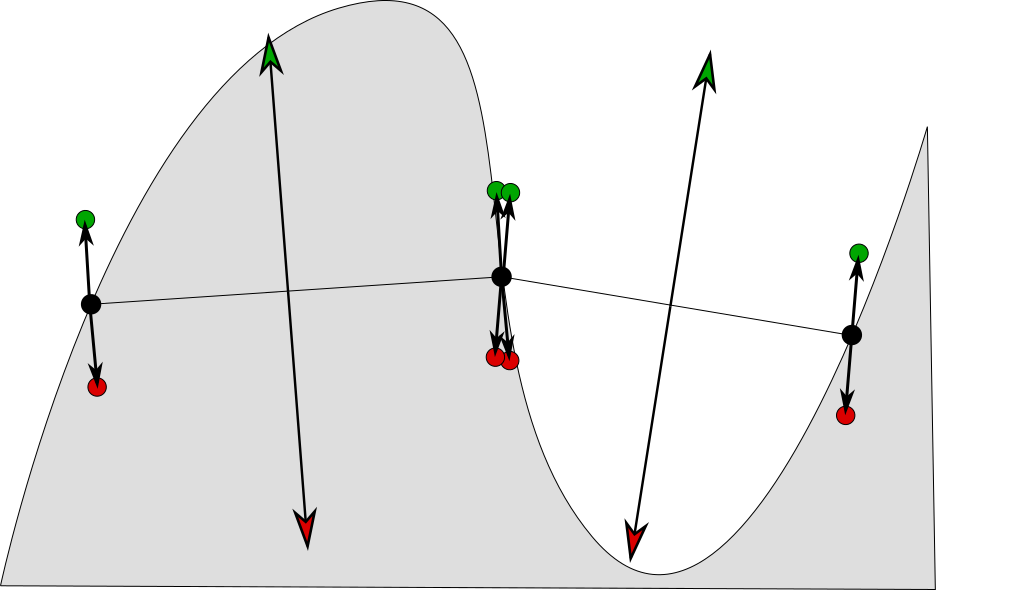
\includegraphics[width=0.55\textwidth]{images/outside_normal}}
        \caption[Počítanie normály trojuholníka ukazujúcej von z plochy]
        {Počítanie normály trojuholníka ukazujúcej von z plochy.}
        %id obrazku, pomocou ktoreho sa budeme na obrazok odvolavat
        \label{obr:outside_normal}
    \end{figure}
}

\item{
    metóda $find\_prev\_next$ v triede $BasicAlgorithm$

    Suseda $x_{prev}$ definujeme ako 
    hraničný vrchol, susedný s vrcholom $x_i$, taký, že uhol $\alpha$ dvoch vektorov
    $\overrightarrow{x_i x_j}$ a $\overrightarrow{x_i x_{prev}}$ vzhľadom 
    na susedný trojuholník $N$ ku hrane $E$ je najmenší. Uhol $\alpha$ definujeme podobne
    ako uhol $\beta$ v kapitole \ref{kap:triangle_conditions} v bode 2 s malou zmenou. 
    \[ 
    \alpha = \left\{
    \begin{array}{ll}
        \beta + 2 \pi & \beta \in \langle -\pi, 0 \rangle\\
        \beta & \beta \in \langle 0, \pi \rangle\\
    \end{array} 
    \right. 
    \]
    
    Suseda $x_{next}$ definujeme analogicky pre vrchol $x_j$ a uhol vektorov 
    $\overrightarrow{x_j x_i}$ a $\overrightarrow{x_j x_{next}}$.

    Ilustráciu môžeme vidieť na obrázku \ref{obr:find_prev_next}, vrchol $x_j$
    má len jedného suseda medzi hraničnými vrcholmi, teda $x_{next} = x_n$. 
    Avšak vrchol $x_i$ má troch
    susedov $x_{p_1}, x_{p_2}, x_{p_3}$. Najmenší uhol $\alpha$ je pri vrchole $x_{p_1}$,
    preto tento vrchol označíme za $x_{prev}$.

    \begin{figure}
        \centerline{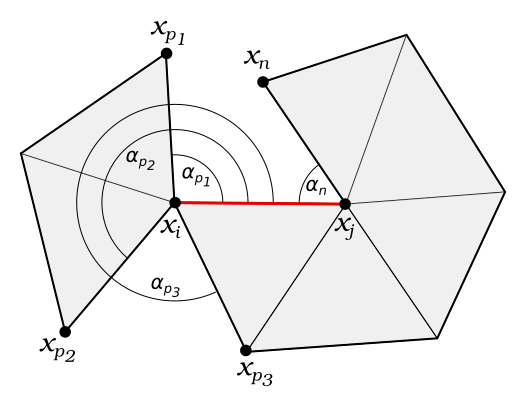
\includegraphics[width=0.5\textwidth]{images/find_prev_next}}
        \caption[Hľadanie susedných hraničných vrcholov]
        {Hľadanie susedných hraničných vrcholov.}
        %id obrazku, pomocou ktoreho sa budeme na obrazok odvolavat
        \label{obr:find_prev_next}
    \end{figure}
}
\item{
    metóda $fix\_corners$ z triedy $BasicAlgorithm$

    Princíp tejto metódy sme opísali v kapitole \ref{kap:bounded_triangulation}.        
    Na začiatku metódy nájdeme medzi ohraničujúcimi hranami tie, ktorých konce neležia
    na tej istej stene. 
    
    Na to využívame nasledujúci postup. Pre oba vrcholy ohraničujúcej 
    hrany vypočítame číslo $f$ reprezentujúce množinu stien, na ktorých daný vrchol leží. 
    Ak si ho predstavíme ako binárne číslo, má jednotku na 1. bite, ak vrchol leží na stene 
    $x_{min}$, na 2. bite, ak leží na stene $x_{max}$, 3. bit patrí stene $y_{min}$, 4. bit
    stene $y_{max}$, 5. bit stene $z_{min}$ a napokon 6. bit stene $z_{max}$. Na ostatných 
    bitoch zostáva 0. 
    
    Potom ak je bitový $and$ týchto čísel pre oba vrcholy nenulový, znamená
    to, že majú nejakú spoločnú stenu. Ak je naopak nulový, neležia na spoločnej stene.
    Zaujímajú nás teda hrany, ktorých bitový $and$ čísel $f_1$ a $f_2$ pre ich krajné 
    vrcholy je 0. Príklad takéhoto výpočtu môžeme vidieť na obrázku \ref{obr:common_faces}, 
    v tomto prípade binárne čísla konvertujeme na decimálne \textit{odzadu}.

    V rámiku naľavo je bitový $and$ nenulový a keďže nenulová číslica je na 5. bite, body ležia
    na spoločnej stene $z_{min}$. V rámiku napravo je bitový $and$ nulový, teda body neležia
    na spoločnej stene.

    \begin{figure}
        \centerline{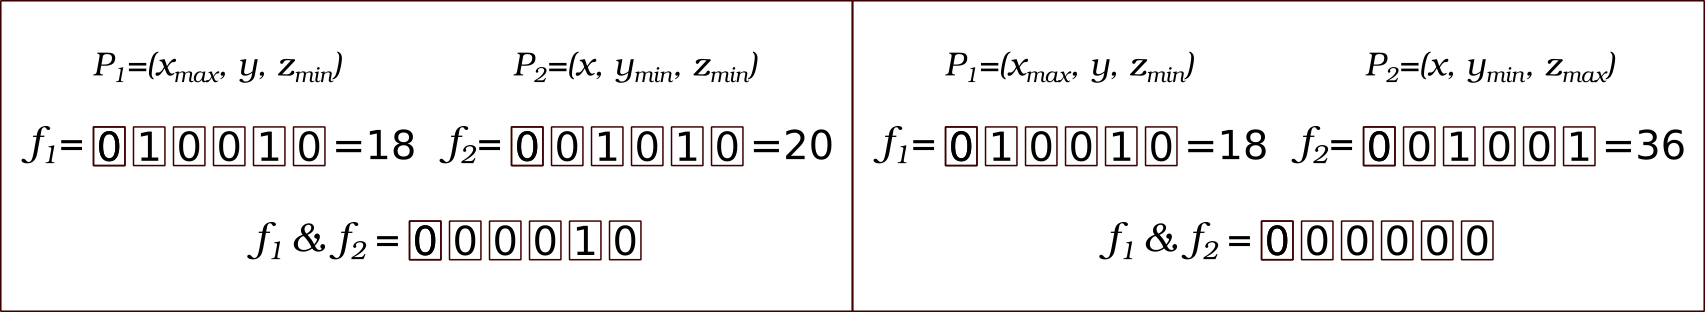
\includegraphics[width=1\textwidth]{images/common_faces}}
        \caption[Hľadanie spoločných stien ohraničujúcich hrán]
        {Hľadanie spoločných stien ohraničujúcich hrán.}
        %id obrazku, pomocou ktoreho sa budeme na obrazok odvolavat
        \label{obr:common_faces}
    \end{figure}

    Pre tieto hrany chceme vytvoriť vrchol, ktorý leží na ploche a zároveň na hrane obálky.
    To dosiahneme premietnutím bodu ležiaceho na blízkej hrane na zadanú plochu v smere 
    smerového vektora tejto hrany. Ako tretiu zo súradníc bodu pre premietanie určíme 
    prislúchajúcu súradnicu stredu hrany $E$. V prípade, že niektorý z vrcholov 
    $x_i$, $x_j$ leží na hrane obálky, vytvoríme nový bod vo vrchole tejto obálky. 

}
\end{itemize}

